\documentclass[12pt, a4paper]{article}

%% Language and font encodings. This says how to do hyphenation on end of lines.
\usepackage[main=english]{babel}
\usepackage[utf8x]{inputenc}
\usepackage[T1]{fontenc}
\usepackage{biblatex}
\usepackage{caption}
\usepackage{multicol,lipsum,graphicx,float}
\usepackage{enumerate}
\usepackage[shortlabels]{enumitem}

\usepackage{ragged2e}

% Keywords command
\providecommand{\keywords}[1]
{
  \small	
  \textbf{\textit{Keywords---}} #1
}
\addbibresource{refs.bib}

%% Sets page size and margins. You can edit this to your liking
\usepackage[top=0cm, bottom=2.0cm, outer=2.49cm, inner=2.49cm, heightrounded,
marginparwidth=1cm, marginparsep=1cm, margin=1.49cm]{geometry}

%% Useful packages
\usepackage{caption}
\usepackage{graphicx} %allows you to use jpg or png images. PDF is still recommended
\usepackage[colorlinks=False]{hyperref} % add links inside PDF files
\usepackage{amsmath}  % Math fonts
\usepackage{amsfonts} %
\usepackage{amssymb}  %
\usepackage{multirow}

\title{Haptic technologies for the Metaverse}
\author{Nathan Poret\\\small{nathan.poret@viacesi.fr}\\\small{Cesi Student FISE SPE INFO
\and {\rm Valentin Pain}\\\small{valentin.pain@viacesi.fr}\\\small{Cesi Student FISE SPE INFO}
\and {\rm Benjamin Brifault}\\\small{benjamin.brifault@viacesi.fr}\\\small{Cesi Student FISE SPE INFO}
\and {\rm Arthur Lecras}\\\small{arthur.lecras@viacesi.fr}\\\small{Cesi Student FISE SPE INFO}
\and {\rm Dove-Steeve Bingo Kpognon}\\\small{dovesteeve.bingokpognon@viacesi.fr}\\\small{Cesi Student FISE SPE INFO}
\and {\rm Pierre Garrido}\\\small{pierre.garrido@viacesi.fr}\\\small{Cesi Student FISE SPE INFO}}}
\begin{document}
\maketitle
\begin{multicols}{2}
\begin{abstract}
The emergence of new technologies and services, nowadays, has broadly led to unique opportunities and ways to personalize user's experience. Regarding IT fields, more data is generated thorough the years, and we are getting closer and closer to create a realistic simulation of human sensations and feelings. However, it is definitely not easy for the client to trust or even to be aware that those technologies exist and can be used at home. Thanks to many researches and scientific experiences, we will try to provide a detailed explanation on how it is, nowadays, possible to simulate senses, and especially the touch through a virtual world. The reader will, as well, be provided feedbacks, particularly about ergonomic and therefore introducing a potential help for the user's decision-making. 
\end{abstract}

\keywords{Metaverse, haptic, ethic, virtual reality, end user}

\section{Introduction}

\par The era of virtual reality has begun. The human senses are beginning to be immersed in another world. Nowadays, the senses able to be simulated are sight and hearing. In addition, other simulations of senses are being developed, such as touch. However, many haptic technologies exist and a choice among them is necessary to perceive which technology will provide the best experience to the user. Knowing this, it is useful to consider the following problematic: which haptic technology is the most suitable for the virtual reality and the metaverse? But first, it is necessary to understand what the haptic technologies can do nowadays? Also, what is the most convenient solution for the end user? And so, do these technologies have drawbacks for the end user? In the first part of this document, we will provide an introduction to the type of tools we can work with today to build a haptic experience. Afterwards, a part will be dedicated to real scientific experiences, hence doing demonstrations and answering some questions the reader may have. Last but not least, a conclusion will be given about our final answers regarding the experiments results and our researches.

\section{State of the art}

\subsection{Augmented Reality, Virtual Reality, and Metaverse}

\subsubsection{Augmented Reality}

\par According to the booklet, “The-Concise-FINTECH-COMPENDIUM” by Patrick Schueffel, p.2: “Augmented reality is an enhanced version of the physical, real-world reality of which elements are superimposed by computer-generated or extracted real-world sensory input such as sound, video, graphics, or haptics.”\cite{AR_def}. So, augmented reality (AR) simulates an additional sensory to the user while that same user is getting its normal and human sensory input from its surroundings.\cite{augmentReal}
\par AR requires a device with a camera and at least one AR software, such as a smartphone, a tablet, or smart glasses, to overlay digital material in a real-world environment. To process the video stream captured by the camera and distinguish objects in the environment, the AR software uses computer vision. Computer vision is a branch of artificial intelligence (AI) that allows computers and systems to extract useful information from digital images, videos, and other visual inputs, as well as to conduct actions or make recommendations based on that data. This enables the AR system to project virtual content in a precise place. The digital content is then realistically shown on top of the real environment via the display device.\cite{metaverse2}
\par Two main types of AR exist: marker-based AR and markerless-based AR. Marker-based AR applications use physical images captured by the camera to place digital content on top of them. Logos, posters, and QR codes are different types of markers. Markerless AR works without artifact and allows users to choose where the digital content is displayed. To obtain information about the environment, markerless-based AR applications use the device's camera, GPS, compass, and accelerometer. It uses three different methods: Superimposition-based AR, Projection-based AR, and Location-based AR. Superimposition-based AR recognizes items in the actual world and partially or completely replaces their original perspective. Location-based AR works in specific places. The virtual object is positioned at the point of interest using the device's GPS and compass. Unlike the previous methods, projection-based AR does not require a display device to display virtual objects, but instead projects light onto a surface to do so.\cite{metaverse2}

\subsubsection{Virtual Reality}

\par Virtual Reality (VR) uses computer technology to build three-dimensional artificial environments that people can interact with. VR technology lets users to be immersed in virtual experiences rather than flat-screen digital experiences using special equipment such as headsets. Unlike AR, which adds virtual objects to the real world, VR provides a more immersive experience and completely simulates an environment.
\par Virtual reality technologies deceive the human brain into viewing the virtual environment as reality by replicating as many senses as possible. Special hardware components are used to achieve this. The main components are head-mounted displays (HMD). HMDs are used on headsets and provide a three-dimensional picture of the virtual environment. It simulates human eyesight with a field of view\footnote{Also called FOV, the observable area a person can see through their eyes or via an optical device.} and a frame rate\footnote{The number of images consecutively displayed each second.}. Another important component are headphones. Headphones provide realistic audio of the environment that matches what the user sees from HMD. To track and adjust the virtual environment, gyroscopes\footnote{Device used to detect the deviation of an object from its desired orientation.}, accelerometers\footnote{Tool that measures proper acceleration (the acceleration of a body in its own space).}, and magnetometers\footnote{Measures the strength and, depending on the instrument, the direction of a magnetic field at a point in space.} are used. They look at the position and the direction of the user’s head in the room to convert them in the simulation. Users can interact with the virtual world using controllers, gloves, treadmills and can stimulate other senses such as touch.
\par The experience of VR can be fully or semi-immersive. A fully immersive VR is the experience that gives the most lifelike experience. It involves all the components used for simulating a sensation, the user is completely cut off from the rest of the real world. The main difference with the semi-immersive VR experience is that the user is not completely isolated from reality and remains connected to their physical surroundings.\cite{metaverse2}

\subsubsection{Metaverse}

\par The term "Metaverse" first appeared in 1992 in the novel "The Virtual Samurai", written by Neal Stephenson. The world described there is a fictional universe, which could be close to our future reality\cite{metaverse2}. The article “Metaverse” by Stylianos Mystakidis gives the following definition: “The Metaverse is the post-reality universe, a perpetual and persistent multiuser environment merging physical reality with digital virtuality. It is based on the convergence of technologies that enable multisensory interactions with virtual environments, digital objects and people, such as virtual reality (VR) and augmented reality (AR).” However, since multiple brands have their Metaverse, there is not only one Metaverse but multiple ones. So, the definition is the same but must be more general, using like “a Metaverse” and not “the Metaverse”.\cite{metaverse2}\cite{metaverse}

\subsection{Haptic technology}

\subsubsection{Origins and Definition}

\par The skin is an extremely complex organ of the human body. In the world of virtual immersion, the sense of touch is essential and allows a more complete immersion of the human mind. This is why haptic devices are becoming more and more important in virtual immersion technologies.
\par A haptic device allows communication between a human and a virtual environment, such as virtual reality or the Metaverse. Also called a tactile-kinesthetic system, this type of device is used to design and manipulate objects with tactile feedback. Video games are equipped with these devices, which lets the controller to produce vibrations related to events and actions in games.\cite{haptic5}
\par For a haptic device to work properly and perform well, it must ideally meet 3 conditions:
\begin{itemize}
    \item Transparency: The user of this device should not feel it being used. The customer should not feel the weight or the friction of the device when handling it.
    \item Position resolution: The device must be able to detect the slightest movement of the user to be able to convert it correctly in the virtual world. If that feature is not perfect, the user might get the sensation of touching an object in the world with the device without actually reaching the object in the virtual world.
    \item Stability: This condition represents the performance of the device to reproduce the sensation of touching an object. Therefore, this condition is the most essential one to develop a haptic device.\cite{haptic3}
\end{itemize}

\subsubsection{Different haptic technologies}

\par Haptic technologies based on vibrations are the most used in the industry today. The sense of touch can be simulated by vibrations, electricity, sound, or heat.
\par The vibrations are produced with the "Eccentric Rotating Mass" (ERM) technology (Figure 1.). This technology is the most widely used to simulate vibrations nowadays. The ERM rotates on itself and when its speed increases, the weight of the eccentric mass becomes unstable and drives the motor into a rotational movement. It is this movement that produces the haptic feedback in the form of a vibration\cite{TBHMI}.

\captionsetup{type=figure}
\centering
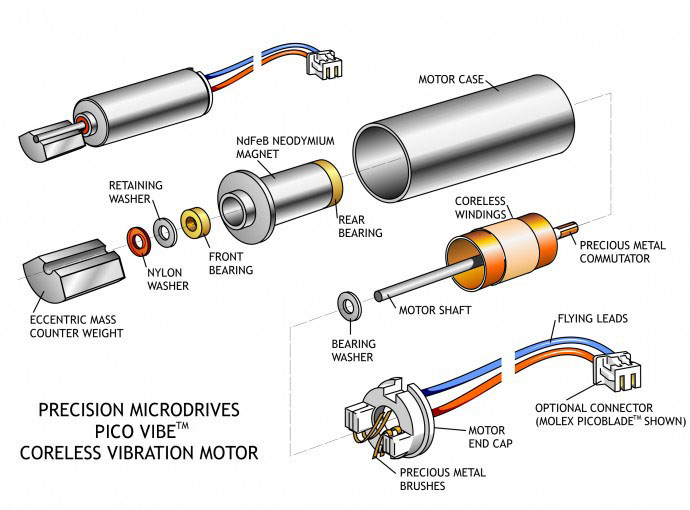
\includegraphics[width=.4\textwidth, ]{ERM.jpg}
\captionof{figure}{Eccentric Rotating Mass (ERM)}
\vspace*{3mm}

\justifying

\par There is also a second technology producing vibrations: "Linear Resonant Actuator" (LRA). This technology is more recent but has already spread in some game consoles like the Nintendo Switch for example. The LRA is composed of a magnet and a spring wrapped in a coil. Once powered on, the coil forces the magnet to move back and forth inside. This movement also produces haptic feedbacks in the form of vibrations\cite{TBHMI} (Figure 2.).

\captionsetup{type=figure}
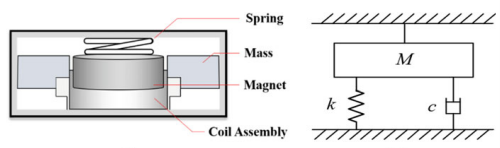
\includegraphics[width=.49\textwidth]{LRA.png}
\captionof{figure}{Linear Resonant Actuator (LRA)}
\vspace*{3mm}

\par Finally, another vibration technology is the piezoelectric actuator\footnote{PZT, transducers that convert electrical energy into a mechanical displacement or stress based on a piezoelectric effect, or vice versa.}. The elementary principle of the piezoelectric actuators is the inverse piezoelectric effect. It can produce deformation\footnote{mechanical stress} when an AC\footnote{Alternative current.} electric field to a piezoelectric material is applied (Figure 3). This deformation is proportional to the intensity of the electric field. Polymers\footnote{Materials made of long, repeating chains of molecules. The materials have unique properties, depending on the type of molecules being bonded and how they are bonded.} are commonly employed in piezoelectric-based force touch-sensing devices due to their excellent mechanical characteristics. However, ceramics are commonly used in haptic applications due to their high piezoelectric coefficient. To transmit the force created by the inverse piezoelectric effect, one side of the piezoelectric material is attached to the mass block. To keep the system stable, the other side is joined to the fixed baseplate. The haptic feedback can be performed by using a high voltage (200 Volts)\cite{TBHMI}.

\captionsetup{type=figure}
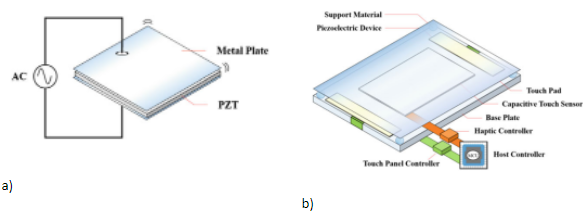
\includegraphics[width=.49\textwidth]{piezo.png}
\captionof{figure}{A piezoelectric actuator, a) A typical piezoelectric actuator structure, b) A capacity touch panel with a piezoelectric actuator by Kyocera Corp with an architecture of 30 Volts (commercial product)}
\vspace*{3mm}

\par This technology provides a short startup time (less than 5 milliseconds) and can reach the programmed acceleration in a short amount of time. When the driven power is used, it consumes less power (from 0.1 to 1 Watts). It is possible to create a more complex haptic effect, by controlling separately the position and the vibration frequency. Moreover, the frequency response range is broad, allowing users to receive the most complete and realistic haptic sensation possible. That being said, a high driving voltage is necessary\footnote{about 200 Volts for four-layer piezoelectric materials.} and the poor boosting efficiency\footnote{35–57\%.} creates significant circuit heating, necessitating the installation of thermal protection for the chip in long-term operations. It requires additional components, and the materials used for PZT are fragile and easily break. And finally, this technology is expensive\cite{TBHMI}.
\par In 2010, Pacinian Corp. introduced a new vibration technology: the surface actuator. This technology distributes, between two plates, positive and negative charges uniformly and uses a spring to limit the movement of the scale (Figure 4.). With that technology, it is possible to create overall vibrations over a vast flat area, users can get keystroke-like effects\footnote{An effect like a single depression of a key on a keyboard, especially as a measure of work.}. On the touch screen, a consistent response can be produced. Also, the system reaction time range is broad, spanning 0 to 500 Hertz. There are no additional actuators necessary to generate vibrations because they are integrated with the touch screen. However, the operating voltage is higher than what we saw in the previous solutions and mass production is still a long way off for now. \cite{TBHMI}

\captionsetup{type=figure}
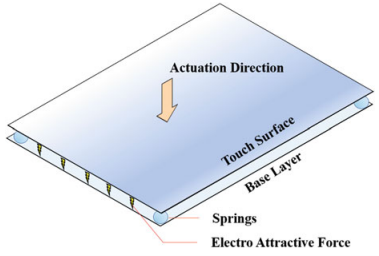
\includegraphics[width=.49\textwidth]{Surface.png}
\captionof{figure}{A surface actuator}
\vspace*{3mm}

\par On the other hand, electroactive polymers (EAP) use electric signal-induced mechanical displacement to provide haptic feedbacks. According to their activation method, EAP actuator's working mechanisms can be split into ionic and electronic-based architectures. High haptic resolution displays have been made using EAP techniques. Each actuator in the display can be manipulated separately to change the display's height, transmittance, and flexibility. Because of its great effectiveness in providing displacements with high spatial precision, EAP techniques are also used for braille reading (Figure 5.). It should be mentioned that EAP technology is still in development, and that various challenges remain unresolved. EAP materials are sensitive to humidity and require the implementation of a water-impermeable surface. Long-term use results in a heavy electrolyte loss phenomenon, which influences surface conductivity. A heat-resistant design is usually chosen to ease the operation at higher voltages without breaking the material's internal structure.\cite{TBHMI}.

\captionsetup{type=figure}
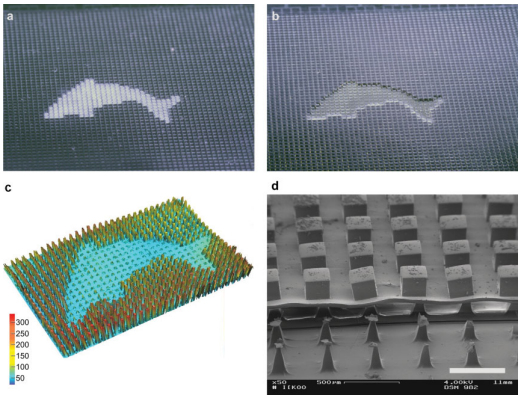
\includegraphics[width=.49\textwidth]{EAP.png}
\captionof{figure}{Generation of visual and palpable information by the "artificial skin" (EAP), a) When the phase transition temperature is exceeded, the hydrogel\footnote{Crosslinked hydrophilic polymer that does not dissolve in water.} immediately changes its color from transparent to opaque. The "artificial skin" displays monochrome visual information; b) After ending the shrinking process, the skin maps the sharp outlines of a dolphin. The length of the dolphin from mouth to tail is 14.49 millimeters; c) The hydrogel actuator array maps the dolphin with sharp contours and single-pixel accuracy; d) In order to improve the palpation of edges and outlines, a knob is placed on top of each actuator.}
\vspace*{3mm}

\par In 2009, Senseg Oy presented "E sense", the first capacitive electro-sensory interface (CEI) method. It uses a short-distance capacitive coupling mechanism to communicate conventional indentation to the skin\cite{TBHMI}.

\captionsetup{type=figure}
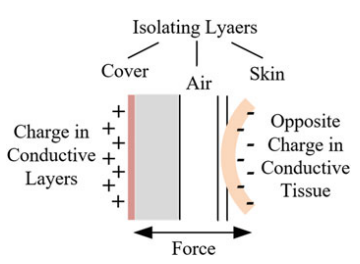
\includegraphics[width=.49\textwidth]{CEI.png}
\captionof{figure}{Working principle of the E-sense when the weakly conductive layer is embedded under the surface of the touch device}
\vspace*{3mm}

\par In that system, the conductive layer is charged during operation and the coupling mechanism causes the opposing charges to accumulate on the finger that contacts the screen surface. Those opposing charges will be attracted to each other by the Coulomb effect\footnote{Coulomb's law states that the electrical force between two charged objects is directly proportional to the product of the quantity of charge on the objects and inversely proportional to the square of the separation distance between the two objects.}, producing a mechanical force (Figure 6.). The vibrational amplitude and frequency can be modified to suit a variety of applications by modifying the polarity and quantity of the charges on the conductive layer and adjusting the frequency of the driving voltage waveform\footnote{The shape of the wave on a graph}. CEI has some benefits: the vibration feedback's frequency, the strength, and the roughness can all be adjusted independently. Also, the finger can hang in the air and communicate both pressure and touch using the principle of short-distance capacitive coupling. However, the effective vibration range is tiny and under sweating conditions, the vibration performance is considerably reduced\cite{TBHMI}.
\par In the article by C. Pacchierotti M. Marchal; G. Gallagher and A. Lécuyer in 2020\cite{virtualReal}, it is demonstrated that focused ultrasound haptics can provide the sensation of interacting with objects of different stiffness.(Figure 7). Indeed, focused airborne ultrasound\footnote{very high intensity and focused mechanical wave.} is the most advanced technology to provide airborne haptics. In this paper, the experiment was performed with an Ultrahaptics STRATOS platform, which is a commercial-focused ultrasound array. An HTC Vive\footnote{One of the most famous and commercialized VR device.} tracker was attached to the participants' dominant wrist to track their hand movement, and a virtual hand avatar mimicked this movement in the virtual environment. In fact, the purpose was to demonstrate the contact ultrasound method of control. This can detect the stiffness of a surface and scan large surface defects such as delamination\footnote{Mode of failure where a material fractures into layers.}\cite{TBHMI}.

\captionsetup{type=figure}
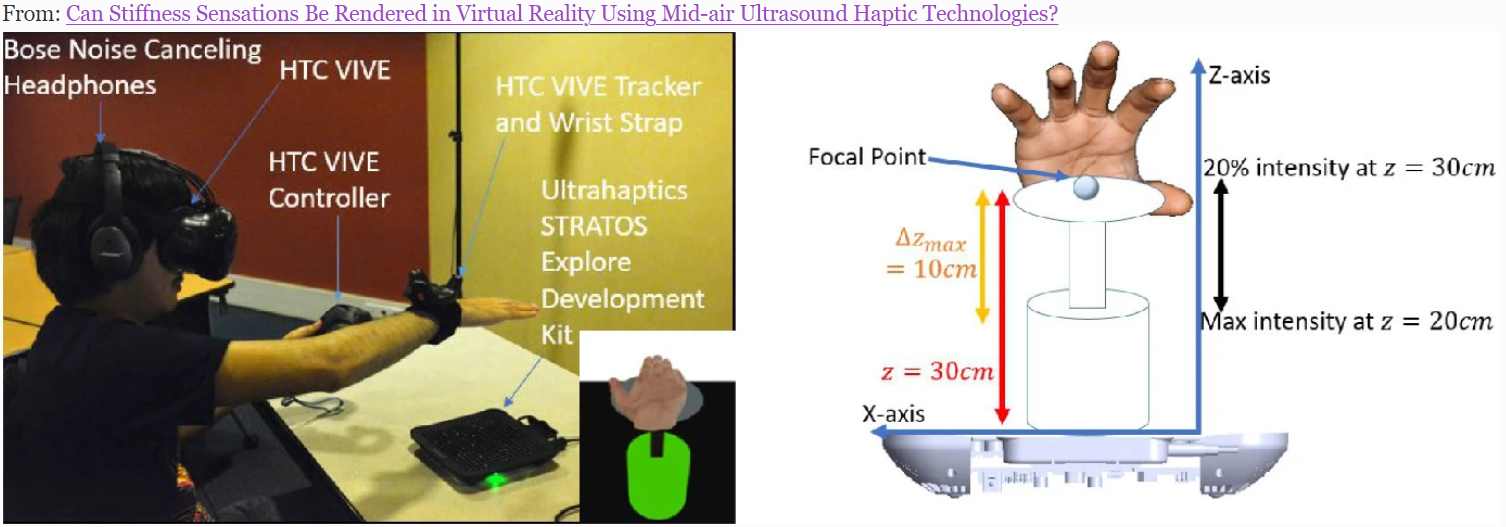
\includegraphics[width=.49\textwidth]{ultrasonic.png}
\captionof{figure}{Ultrasonic technology}
\vspace*{3mm}

\par Electrical muscle stimulation, also known as electrostimulation, is a technique for stimulating muscles through electrical impulses of varying degrees. Indeed, when the muscle receives electricity, it contracts and sends information about its condition to the brain. Thanks to this method, first used in the medical field, it is possible to simulate a virtual environment while having haptic sensations linked to the virtual actions carried out by the user.
\par The sending of electric current to the muscles is done thanks to electrodes simply stuck on the skin\cite{virtualReal}(Figure 8).\newline

\captionsetup{type=figure}
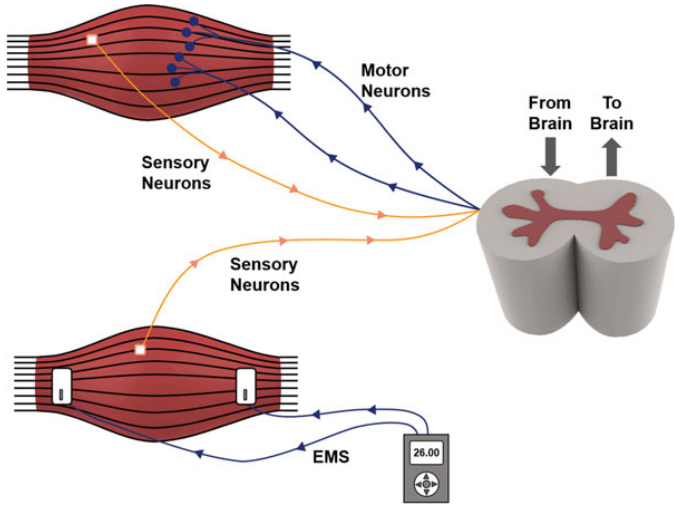
\includegraphics[width=.49\textwidth]{EMS.png}
\captionof{figure}{Electro-Myo-Stimulation (EMS)}
\vspace*{3mm}

\par The study on bioelectrical stimulation published in Shuo GaoShuo, YanHang Zhao and Arokia Nathan's book shows that the bioelectrical stimulation technique can improve the performance of the interaction between the human and the machine. Indeed, the haptic feedback results in the activation of the muscles by the electrical pulses. In addition, the biological study that benefits the development of functional electrical stimulation shows the composition of the sensory receptors of human fingers. In fact, the so-called Axon receptors are of the fast-adapting type, the slow adapting type I\footnote{SA1, mechanoreceptor with the Merkel corpuscle end-organ, underlies the perception of form and roughness on the skin} and the Pacinian corpuscle\footnote{Onion-shaped structure of nonneural (connective) tissue built up around the nerve ending that reduces the mechanical sensitivity of the nerve terminal itself.}\cite{TBHMI}.
A technology using neuromuscular stimulation all over the body is called a haptic suit. Using built-in sensors, the suit stimulates the muscles and produces the feeling of touch on the body\cite{hapticexperience}. That haptic system allows motion capture, temperature control and biometric monitoring. Electrostimulation is used to simulate heat and cold sensations on the body. The commercialized "Teslasuit" is, nowadays, a good example of what humans can do with haptic suits\cite{teslasuit} (Figure 9.).\newline

\captionsetup{type=figure}
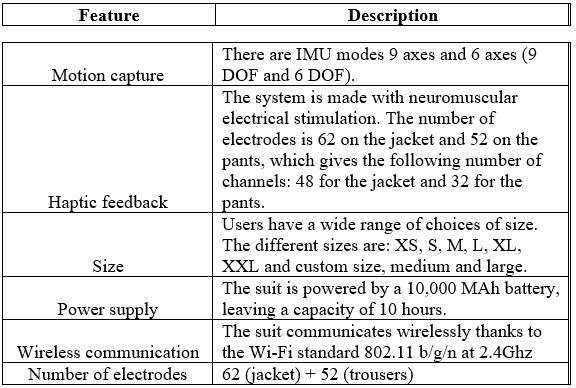
\includegraphics[width=.49\textwidth]{tableau-haptic-suit.PNG}
\captionof{figure}{Teslasuit Features Chart}
\vspace*{3mm}

\par These different cells have well-defined functions. The fast-adapting axons\footnote{Also called nerve fibre, the portion of a nerve cell (neuron) that carries nerve impulses away from the cell body.} are the closest to the superficial skin and the slow-adapting type I is the second closest, while the Pacinian corpuscle is the deepest. Indeed, the axons are stimulated from the inside and outside as the potential inside the axon is relatively stable, the activation force is directly associated with the potential outside. In addition, this technology uses electrodes to inject current through the skin, and at the same time generates pressure and vibration sensations to achieve haptic feedbacks\cite{TBHMI} (Figure 10.).

\captionsetup{type=figure}
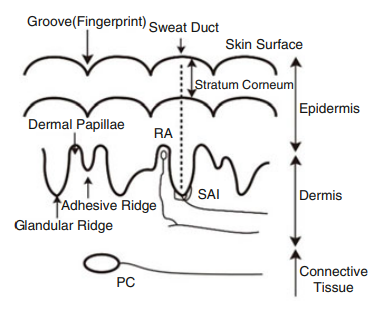
\includegraphics[width=.49\textwidth]{FES.png}
\captionof{figure}{Functional Electrical Stimulation (FES)}
\vspace*{3mm}

\par In the article from TechXplore written by Steve Kuhlman, the research team explains that a feeling provided by the friction during a contact with a touchscreen can be modified by changing locally the temperature. So, they will be able to reproduce some texture like “the skin of a snake” or “fabric of clothes”. They explain that there is a unique couple of mechanical and thermal sensations associated with a specific texture. The application domains are very varied and are very interesting for the Metaverse. They didn’t give any details about how it works because the research is just starting, many difficulties remain as well as things to discover. For example, the miniaturization and the integration for touchscreens will be a great challenge\cite{haptic7}\cite{hapticTemperature}.

\subsection{Ethics in the Metaverse}

\par Advances in virtual reality technology allow for a more immersive, realistic, and better experience of the Metaverse. The Metaverse uses data collected in the real world to offer immersive experiences. This virtual universe that this new technology offers, gives the possibility to be in a world that is getting closer and closer to the real world. With the arrival of haptic technologies, users can interact with other assets and virtual avatars. A haptic virtual reality suit allows users to feel physical contact sensations all over their body while immersing themselves in virtual reality. However, the relationships and social interactions can interfere users' habits, activities, and choices in the Metaverse\cite{ethics}.
\par The reality devices that the Metaverse incorporates can therefore capture a large amount of information, from users' biometric data to spatial data, including environments such as the physical space around the Earth. It goes without saying that a real ethical problem arises\cite{ethics}.
\par The approach of recent activities conducted on the ethical issue of the Metaverse reveals concerns related to the vulnerability of certain groups of people, the interactions between users, the after-effects of the consumption of haptic technologies, the confusion between real and virtual, data issues, the Metaverse as an interface to inflict physical harm, and the potential psycological and social implications\cite{ethics}.
\par Indeed, the framework and level of freedom are not yet clearly defined, so privacy is at risk. The Metaverse can collect certain biometric data and the various movements made, preferences, places visited... that are not obvious to users. The collected biometric data endangers the most personal aspects of our existence\cite{ethics}.
\par Moreover, as we have noted earlier, liver technologies allow sensory feedback. This creates a huge ethical problem because any virtual contact is reflected in the physical body. Indeed, the sensors attached to the users can realistically control their avatar. The Metaverse cannot control the psychological state of the users, so the users are not safe from virtual aggression on the avatars, which reverberates on the physical body\cite{ethics}.
\par The development of more and more realistic virtual worlds with the concept of the Metaverse allows us to use the progress of the technology, including the sensory return with the haptic technology. This peculiar technology creates an ethical problem, essentially based on privacy, since it collects biometric data to make the user's experience in the Metaverse more realistic\cite{ethics}.
\par In general, the Metaverse can easily become an ethical problem in the management of personal data.
\par The increase in realism by the Metaverse technology can be explained by the rise of personal data acquisition through haptic technologies. To improve the movement's fluidity of the avatars, it is necessary to activate others useful functionalities, like the location of the user in his room and the motor actions to virtually reproduce the movement. Many more information can be recorded such as traits, motor actions, eye movement patterns, reflexes, preferences and habits\cite{ethics}.
\par This type of personal data cannot normally be collected by current products or experiences without this technology being integrated into current consumption patterns. New ways of thinking are therefore needed to address the collection of data specific to haptic technologies\cite{ethics}.

\section{Experiences and Demonstrations}

The state of the art has shown us that current haptic technologies can reproduce a large number of different sensations such as weight, temperature and collisions and, must respect some ethical measures. In the next part, we will discuss and show the results of scientific experiences to test and verify the technologies that we just presented.

\subsection{Simulate haptic sensation using sound}

\subsubsection{An additional feeling}

In order to reproduce the sensation of touch accurately, it must be carried by a sound after each action. To demonstrate the effectiveness of realism of the sound, the document “Audio-haptic physically based simulation of walking on different grounds” states that “In the development of multimodal environments such as games and virtual reality installations, walking sounds are often used to produce physicality and a sense of action, with the overall goal of heightening the realism of a character or person.” \cite{soundAndHapic}. The authors of this paper conducted the experiment using shoes with a pressure sensor and two integrated vibrations-based actuators in each of them. The actuators were fixed under the toe and the heel to enable proper vibration transfer inside the soles (Figure 11.).

\vspace*{3mm}
\captionsetup{type=figure}
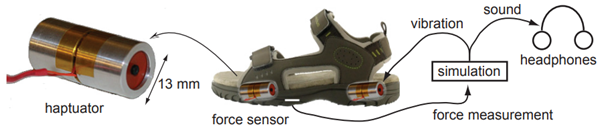
\includegraphics[width=.49\textwidth]{System_hapic_and_sound_experiment.png}
\captionof{figure}{System (one shoe shown). Left: recoil-type actuation from Tactile Labs Inc. The moving parts are protected by an alumimum enclosure cable}
\vspace*{3mm}

The actuators were all powered by the same signal, but they could be developed separately to highlight front or rear activation, strike a balance, or achieve other effects like modulating various back-front signals during heel-toe movements. Algorithms simulating the sounds of people walking on different surfaces were used. So, they were able to simulate a real-time footfall synthesizer that provides audio and haptic feedback. “The developed system is ready to be integrated in computer games and interactive installations where a user can navigate.”\cite{soundAndHapic}.

\subsubsection{Shockwaves for Haptic Sensations}

The use of other means of providing haptic sensations was largely inspired by Yanagida's air gun, which led to the exploration of loudspeaker-based air cannons\cite{soundAndHapic2}. In the paper “Experiences of using Shockwaves for Haptic Sensations” (2005), experiments have been carried out using the iCone. The iCone is a spherical screen about 7 meters in diameter and has a field of view of 210 degrees, with slightly sloping walls (7 degrees towards the back), giving it a conical shape. The iCone has 16 speakers that were placed in a spherical setup, in a top and bottom ring. The sound will produce a vibration through the body and give a sensation of touch. The results were not as good as expected, in fact, the document state the following sentence : “Users especially report on the effects of the sound floor – acoustic effects like a heartbeat in a medical demo can be clearly experienced via vibration.”, but : “Most users do not directly realize the haptic effects of the system”. The vibrations of the floor, which are generated by both the subwoofers and the Paraseats\footnote{Commercialized type of emphaser.}, jolt the user's body, causing mild but distinct sensations in the stomach and chest. Most haptic effects appear to be caused by vibrations sent from the feet through the user's bone structure. Some effects cannot be reproduced, such as the blast effect because this requires a sudden increase in volume from 1 to 80 decibels and can cause health problems to the user such as drowsiness or stomach problems\cite{ISO-vibration}. Finally, “The validity of the vibrations therefore mainly seems to be to enhance a sound system by making sound effects tactile”. The tactility can be used to simulate the effects of collisions, such as colliding with a wall. The vibration also appears to provide motion clues. The most likely reason for this effect is that vibrations beyond a particular level (90 decibels) cause motion feelings in a portion of the inner ear\cite{soundAndHapic2}. The main problems with that solution are its size, its inability to produce certain effects that may not be harmful to health, and unexpected motion sensations because of vibrations in the inner ear.

\subsection{Nerves stimulation}

Several studies have shown that haptic stimulation is closely related to a user's sense of sight. Indeed, a user will be more likely to focus his attention on the active tactile area.\cite{humancomputer}.
Different body areas have been tested to determine which ones are more likely to accept and optimize the results of a haptic sensation by vibration\cite{humancomputer}.

\vspace*{3mm}
\captionsetup{type=figure}
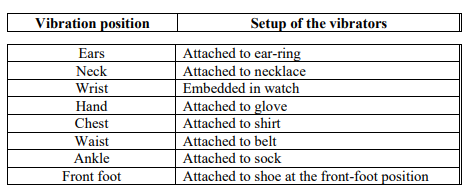
\includegraphics[width=.49\textwidth]{vibrators.png}
\captionof{figure}{Setup of vibrators for each vibration position}
\vspace*{3mm}

Experiment 1 is the most interesting of the study in this case because it determines which areas of the human body are most sensitive to haptic technologies. To perform this experiment, 10 subjects (7 males and 3 females) between 20 and 26 years old was required. The vibrations can go up to 1200 rpm\footnote{Revolutions per minute, number of turns in one minute.} at a frequency of 200 Hertz. The procedure of the experiment was respected, each user positioned the different vibration systems on his body (Figure 12.) and kept them during the 3 tests without changing their place. Each vibration took place every 2.5 seconds. After each vibration, the users were asked to rate their sensation from 1 to 7 on the Likert scale\footnote{Question that uses a 5 or 7-point scale, sometimes referred to as a satisfaction scale, that ranges from one extreme attitude to another.}. 1 being the most difficult to feel and 7 being the easiest to feel\cite{humancomputer}.

\vspace*{3mm}
\captionsetup{type=figure}
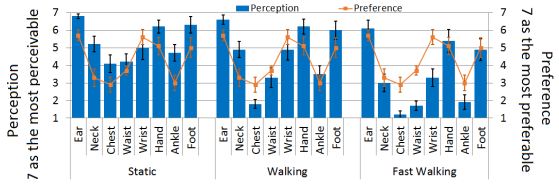
\includegraphics[width=.49\textwidth]{Perceivability.png}
\captionof{figure}{Perceivability ratings (with standard error bars) for each of 8 vibration positions, user preference ratings for each vibration position}
\vspace*{3mm}

The results show that the users' preferences are mainly the ear, hand and wrist (Figure 13.). In contrast, the neck, waist, ankles, and chest are areas that have more difficulty perceiving vibrations. Some participants were asked to comment on the experience, and most of them stated that vibrations in the neck area are very uncomfortable. One user also proposed the idea of developing a vibration ring to wear around the fingers for muscle and nerve stimulation in the hands\cite{humancomputer}.

\vspace*{3mm}

Another experiment presented at the World Haptic Conference (WHC) aimed to test haptic stimulation on the head, neck or back using several actuators and tools to track the movements of the user's eyes. For this experiment, 20 volunteers student between 20 and 37 years old were chosen. The hardware used for this experiment was a T60 eye tracker from Tobii Technologies and C2 actuators from Engineering Acoustics\cite{whc}.
The participants in this study were equipped with 2 sensors on the sides of their forehead, 2 sensors on the neck and 2 sensors on the back. All sensors were calibrated to detect the user's direction of motion and eight directions. Two different methods were used, first, the sensors were activated for 100 milliseconds sequentially, with an interval of 150 milliseconds. The second method was to activate the sensors in a parallel way - i.e. all the sensors were activated during 100 milliseconds at the same time\cite{whc} (Figure 14.).

\vspace*{3mm}
\captionsetup{type=figure}
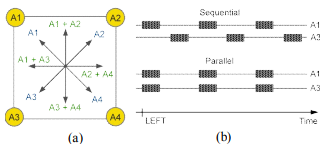
\includegraphics[width=.49\textwidth]{StimulationModel.png}
\captionof{figure}{Stimulation model (a) and a signal timing for the encoded direction “left” in sequential mode (b).}
\vspace*{3mm}

The participants then had a few minutes to understand how the eye tracker works and to feel the vibrations correctly in order to recognize which type of vibration corresponds to each direction. Once the calibration was completed, the users saw a red square appear in the center of the screen, they had to look at it and after 2.5 seconds, several blue squares appeared. The participants were instructed to look at the blue squares that the screen selected\cite{whc} (Figure 15.).

\vspace*{3mm}
\captionsetup{type=figure}
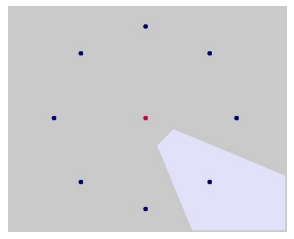
\includegraphics[width=.49\textwidth]{ExperimentalSetup.png}
\captionof{figure}{Experimental setup, software: red home-box (visible before each trial) and blue targets (the focus cone was visible only during the practicing session)}
\vspace*{3mm}

Each square viewed by participants was recorded for future comparison\cite{whc}.

\vspace*{3mm}
\captionsetup{type=figure}
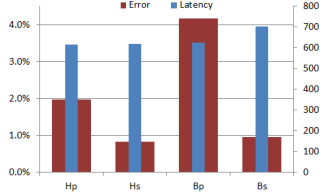
\includegraphics[width=.49\textwidth]{DataResults.png}
\captionof{figure}{Pointing error (\%) and reaction latency (milliseconds) of each simulation}
\vspace*{3mm}

\begin{tabular}{r@{: }l r@{: }l}
H & head and neck\\B & back \\p & parallel stimulation\\s & sequential stimulation
\end{tabular}
\vspace*{3mm}

The analysis of the results shows that sequential vibration stimulation at the head and neck level and sequential vibration stimulation at the back level have a low error rate compared to parallel vibration stimulation at the head and neck level and parallel vibration stimulation at the back level (Figure 16.). It is therefore possible to conclude that parallel stimulation is the most stimulating for the human brain\cite{whc}.
On the other hand, this paper tries to demonstrate the best technical solution for the user of a store having the possibility to touch the virtual clothes. That way, it is necessary that the haptic stimulation is parallel to the user's actions. According to this study, it is then possible to use a haptic headset that stimulates the user's actions in the real world thanks to sensors placed on his neck and head. Indeed, the first column of the above graph represents the most useful case for the current study because the error rate remains relatively low as long as the latency rate can be decreased by increasing the vibration power to reasonable rates\cite{whc}.

\subsection{Haptic gloves, mechanical, vibratory and heat sensation}

As we have said in our paper, haptic feedback allows us to simulate the sensations of touch. These sensations are perceptible in interactive experiences such as virtual reality, for instance, but also in other experiences such as increased virtual reality or the metaverse, or even a combination of the two. 

Most of the experiments that have been carried out highlight the use of mechanisms that can simulate this sensation of touch. Thanks to different sensors, haptic gloves, for example, can offer a sensation of finger resistance on an object\cite{hapticglove}.

Micro-vibrations can simulate different textures at the fingertips\cite{hapticaptor}. These mechanisms greatly increase immersion in virtual reality and are also used on full suits\cite{hapticsuit}. 

The experiment in the paper Smart Tactile Gloves for Haptic Interaction, Communication, and Rehabilitation (2020-2021)  shows that a multimodal sensing and feedback glove is developed with flexible, stretchable, lightweight and compact sensor and heater sheets made by direct ink writing of a liquid metal, eutectic gallium-indium. In the sensor sheet, ten sensors and three vibrators are integrated to measure finger movements and provide vibro-haptic feedback. The other heated sheet provides accurate and fast thermo-haptic sensation via pattern-based feedback control, even under stretched conditions. The multi-modal sensing and feedback glove allows users to feel the contact state and distinguish materials\cite{hapticglove1}. 
The most interesting products in that document are the smart gloves based on gesture and touch (Figure 17.). These gloves are very useful in many different areas, such as telemanipulation, medical/military training, virtual collaborative product design, smart manufacturing, gaming, entertainment, and product advertising. This type of glove uses a resistive fabric-based material and doesn’t need any actuator material. It needs a supply power of 227 milliwatts and is able to use Wi-Fi as a wireless communication protocol\cite{hapticglove1}.

\vspace*{3mm}
\captionsetup{type=figure}
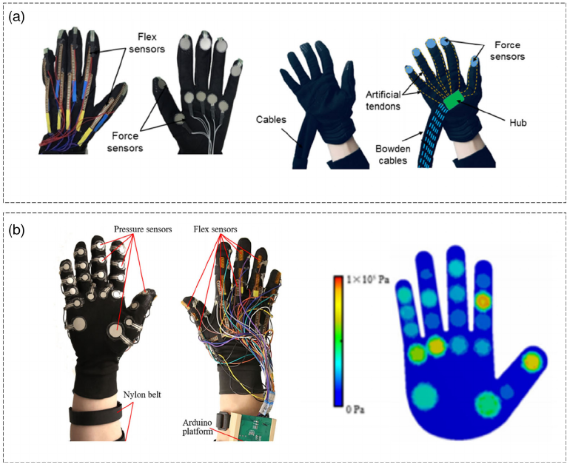
\includegraphics[width=.49\textwidth]{gloves-gesture-touch.png}
\captionof{figure}{Smart gloves combining gesture and touch. a) Wearable hand rehabilitation system with soft gloves: this glove recognizes touch at certain points on the fingers and palm, as well as measuring finger bending angles for gesture recognition. b) Pressure and flex sensors are used in this glove to define fine hand movement.}
\vspace*{3mm}

Those gloves were tested and used for badminton, but they could also be used in other VR/AR applications. The glove does a good job of conveying the feel of the ball bouncing off the badminton racket. It is said to be comfortable and easy to wear. That being said, users had some difficulties to put it on and is described as fragile, the sudden movements are to be avoided\cite{hapticglove1}.

Using an haptic suit in conjunction with gloves will provide more realistic feelings. It lets users feel almost every interaction in the virtual environment.

\subsection{Simulation of haptic sensation by stimulating neural activity}

Haptic simulation can also be recreated by stimulating neural networks. In the document “An artificial sensory neuron with visual-haptic fusion”, they state that “biological systems always outshine their electronic counterparts due to their sophisticated sensorimotor skills”, also, they claim that biological systems have a “superior fault tolerance and power efficiency are inherent in the adaptive, plastic, and event-driven network of sensory neurons.”. Knowing that, simulating biological processes at the level of sensory neurons would enable biological perceptual skills to be realized \cite{neural-haptic}.
To experiment the sensations of touch and vision, a bimodal artificial sensory neuron (BASE)\footnote{Can collect optic and pressure information from the photodetector and pressure sensors respectively, transmits the bimodal information.} has been developed. This neuron is based on a hybrid ionic/electronic neuromorphic electronics. This BASE unit consists of four core components: resistive pressure sensor\footnote{Utilizes the change in electrical resistance of a strain gauge bonded to the diaphragm that is exposed to the pressure medium.}, perovskite-based photodetector\footnote{Combines effective light absorption in the broadband range with good photo-generation yield and high charge carrier mobility}, hydrogel-based ionic cable, and a synaptic transistor (Figure 18.).

\vspace*{3mm}
\captionsetup{type=figure}
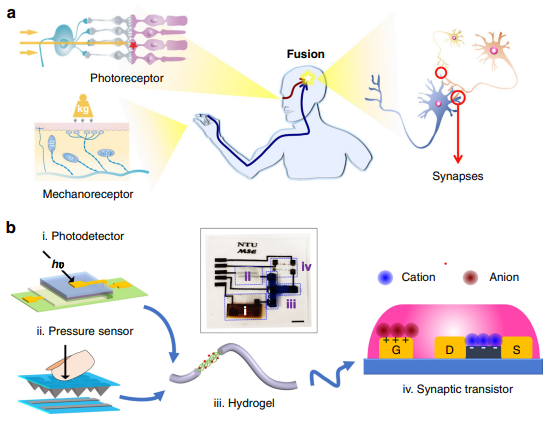
\includegraphics[width=.49\textwidth]{neural-haptic.png}
\captionof{figure}{A bimodal artificial sensory neuron with visual-haptic fusion. a) The visual-haptic fusion by biological neural network. b) The BASE patch for visual/haptic fusion. Sub-figures i to iv: photodetector, pressure sensor, hydrogel, and synaptic transistor, respectively.}
\vspace*{3mm}

External haptic and optical cues are converted into electrical signals by the photodetector\footnote{Device that converts incident light or other electromagnetic radiation in the UV, visible, and infrared spectral regions into electrical signals.} and pressure sensor, which are receptors in the retina and skin. The electrical signals from the two sensors are then sent to the synaptic transistors via the ionic cable, where they are combined and converted into a transient channel current. Bimodal stimuli are used to offer multidimensional spatial information, allowing a biohybrid neuromuscular junction or a robotic hand to be controlled, simulating the "perception for action" process\cite{neural-haptic}.

The hybrid neural circuits are essentially characterized by the visual channel and the haptic channel. The visual channel comprises a perovskite-based photodetector and represents the photoreceptors of the human retina. These photoreceptors are stable in the environment for reliable and repeatable photodetection. The haptic channel is composed of a pressure sensor that incorporates microstructures in the top layer of poly-coating\footnote{Layer applied to the surface of a substrate for the purpose of protecting it.}. Experimental results show that when pressure is applied to the top layer, it forms a resistive path with the electrodes of the bottom layer. Increasing the pressure increases the contact area, and this has an inverse effect on the resistance. The information from the two artificial sensory channels is carried by the ionic cables, which perform the function of an ionic transmission\cite{neural-haptic}.

Furthermore, the development of the ionic hybrid, mimicking the supermodal sensory fusion in the sensory nervous system, combines optical and pressure stimuli to generate biological excitatory postsynaptic currents through the synaptic transistor. The time-dependent bimodal information carried by this current is like neural behaviour. This signal is used to innervate skeletal myotomes\footnote{The muscles served by a spinal nerve root.} and provide information for the movement of robotic hands, for example. This mimics the control of movement by using bimodal sensory signals at the unimodal cellular level.
The bimodal artificial sensory neuron (BASE) is characterised by a sensory modality based on pressure and light, and it uses the 15 millimeters myotube as an actuator. In addition, the size of its action is 5 micrometers and its recognition mode is multi-transparency with dendritic\footnote{Dendritic cells are a type of antigen-presenting cell (APC) that form an important role in the adaptive immune system.} integration constituting synapse emulation\cite{neural-haptic}.

\subsection{Data transmission}

The representation of a haptic signal can be massive, the transmissions of this signal by the network will then be a key point for the user. However, the number of transmitters for a combination can also be important. The problem here is that the weight of these signals is proportionally more important.
C. Shahabi, A. Ortega and M. Kolahdouzan (in 2002) used a method with sampling\cite{shahabi_comparison_2002}. They calculated an ideal sampling rate to reduce the amount of information on a haptic signal. They then calculated the loss rate after signal reconstruction. It is the combination of ADPCM\footnote{Compression coding using differential values where the quantization stages scaling is adapted additionally based on the signal curve.} and AS\footnote{Adapting selection criteria as the experiment progresses, based on preliminary results as they come in.} that showed interesting performances with a substantial reduction in storage requirements while maintaining low error distortion.

Y. You and M. Y. Sung (2008) calculated the throughput\footnote{Rate of successful message delivery over a communication channel, such as Ethernet or packet radio.} for sending haptic device coordinates using the floating-point compression method\footnote{Precise compression method that can require large data spaces.}\cite{you_haptic_2008}. In their experiments, they measured the throughput of six different actions: static, slow, star pattern, figure eight patterns, irregular, and a motion without compression. The results show that the actions compressed with the floating-point method use less throughput.

The previous two experiments exploit two different compression methods : the combination of ADPCM and AS for signal strength and the floating-point to compress the coordinates. We will take into consideration that criteria and the results of the experiences above to compare the most used haptic solutions nowadays.

\subsection{Results comparison}

\captionsetup{type=figure}
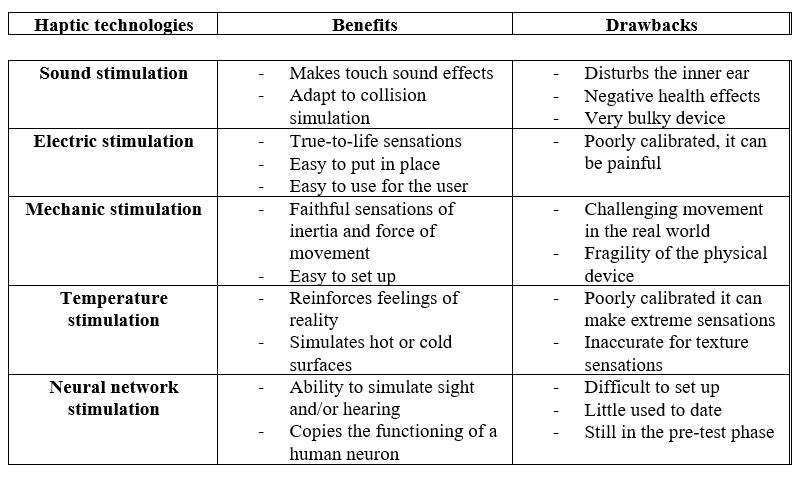
\includegraphics[width=.49\textwidth]{comparison.png}
\captionof{figure}{Comparison of haptic technologies}
\vspace*{3mm}

All these different haptic technologies make it possible to experience a virtual sensation in the real world. However, some of these technologies have bigger drawbacks than others (Figure 19.). Sound stimulation can be dangerous for health, mechanical stimulation is too fragile to be manipulated according to the main problem, neural stimulation is still too experimental to be marketed, and finally, temperature stimulation does not faithfully transcribe textures and is not suitable, once again, to the main problem. The table above highlights the fact that these solutions are not suited for an end user buying a service and using the technology at home. That being said, our comparison does not mean that these are not used at all in scientific fields.

\vspace*{3mm}

Electrical stimulation, on the other hand, makes it possible to stimulate an environment fairly faithfully and is not as fragile. It is also widely used in virtual simulation and is no longer in the pre-test phase. Finally, it has no negative effects on health thanks to the regulation of electrical impulses, which makes it a nice candidate for a client.

\section{Conclusion}
The sensation of touch in virtual reality can be simulated by many haptic technologies. Those can be based on vibration, heat, sound waves or even electrical impulses. Despite the progress of these technologies nowadays, none of them are yet commercialized and all of them must be improved in the following years. That being said, we can clearly see some haptic technologies and improvements being used at home in the upcoming years. Nonetheless, this can only work if the solution for the end-user is usable through networks and understands the major ethic problems of nowadays. 
\newline Experiences have shown that eletrical stimulation is the best option today for a great experience regarding the end user since it has no negative consequences in comparison to other solutions such as sound, mechanical or temperature simulation. Electrical stimulation is also relatively easy to be implemented and provide accurate haptic sensations as long as the ethic aspect is taken in account. It is important to say here that the other solutions approached in this article are still valid for many fields but do not really suit for an immersive user experience, especially in systems like VR and metaverses.
Our team already see the potential behind this solution and especially in some fields related to services such as fashion, social medias, or even military. In the future, neuronal solutions seem to be conclusive and scientists are positives that new technologies and services will soon emerge in that specific field.

\printbibliography
\end{multicols}
\end{document}

https://dl.acm.org/doi/abs/10.1145/2993148.2993171
https://onlinelibrary.wiley.com/doi/full/10.1002/adfm.202008831
https://link.springer.com/chapter/10.1007/978-3-030-58147-3_3 3
https://ieeexplore.ieee.org/document/5444645
https://ieeexplore.ieee.org/abstract/document/4140943
https://www.researchgate.net/publication/319096104_Concept_and_application_of_virtual_reality_haptic_technology_A_review
https://www.sciencedirect.com/science/article/pii/S2214785317303188
https://ieeexplore.ieee.org/document/9382898
https://www.science.org/doi/10.1126/scirobotics.abl4543
https://dl.acm.org/doi/abs/10.1145/2480741.2480751
https://www.mdpi.com/2673-8392/2/1/31/htm
https://web.archive.org/web/20180425130029/http://www.heg-fr.ch/FR/HEG-FR/Communication-et-evenements/evenements/Documents/Schueffel2017_The-Concise-FINTECH-COMPENDIUM.PDF
https://link.springer.com/book/10.1007/978-3-030-68948-3
https://techxplore.com/pdf565546722.pdf